\documentclass[tikz,border=2pt]{standalone}
\usepackage{amsmath,amssymb}
\usepackage{pgfplots}
\pgfplotsset{compat=1.18}

\begin{document}
% The expectation is the balance point of the probability mass: with masses 0.1, 0.2, 0.3,
% 0.4 at 1, 2, 3, 4 the pmf balances at E[X] = 3.
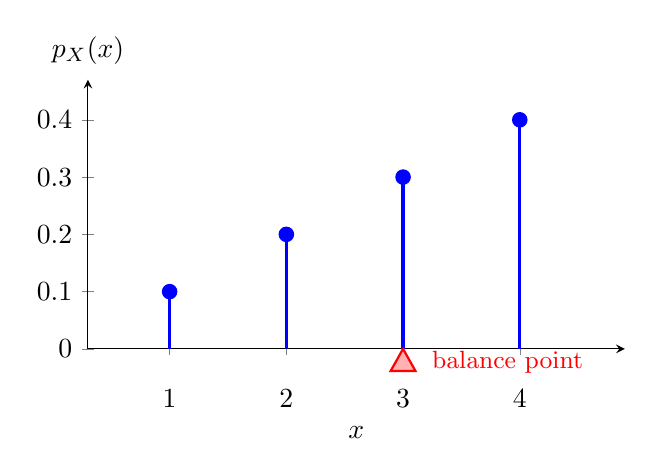
\begin{tikzpicture}
	\begin{axis}[
		axis lines=left, xmin=0.3, xmax=4.9, ymin=0, ymax=0.47,
		xtick={1,2,3,4}, ytick={0,0.1,0.2,0.3,0.4}, xticklabel style={yshift=-9pt},
		xlabel={$x$}, ylabel={$p_X(x)$}, ylabel style={rotate=-90, anchor=south, at={(axis description cs:0,1.02)}},
		width=8.4cm, height=5cm, clip=false
		]
		\addplot[ycomb, blue, very thick, mark=*, mark size=2.2pt] coordinates {(1,0.1) (2,0.2) (3,0.3) (4,0.4)};
		\draw[red, thick, fill=red!30] (axis cs:3,0) -- ++(-4.5pt,-8pt) -- ++(9pt,0pt) -- cycle;
		\node[red, anchor=west, font=\small] at ([xshift=7pt,yshift=-5pt]axis cs:3,0) {balance point};
	\end{axis}
	
\end{tikzpicture}
\end{document}
